\documentclass[conference]{IEEEtran}
\usepackage{amssymb,amsmath}
\usepackage{graphicx}
\usepackage{tabularx}
\usepackage{subfigure}
\usepackage{algorithm}
\usepackage{algpseudocode}
\usepackage{epstopdf,mathrsfs}
\usepackage{hyperref}
\usepackage{xspace}
\newtheorem{theorem}{Theorem}
\newtheorem{definition}{Definition}
\newtheorem{notation}{Notation}
\newtheorem{proposition}{Proposition}
\newtheorem{lemma}{Lemma}

\newcommand{\NP}{\mbox{${\cal NP}$}}

\algnewcommand{\And}{\textbf{and}\xspace}
\algnewcommand{\Or}{\textbf{or}\xspace}

\begin{document}

\title{\LARGE A Novel Algorithm for Thermal-Constrained Energy-Aware Partitioning in Heterogenous Multiprocessor Real-Time Systems}

\author{\IEEEauthorblockN{Bj\"{o}rn Barrefors, Ying Lu, Shivashis Saha, and Jitender S. Deogun}
\IEEEauthorblockA{Department of Computer Science and Engineering, \\
University of Nebraska-Lincoln,
Lincoln, NE 68588-0115, U.S.A. \\
Email: \{bbarrefo,ylu,deogun\}@cse.unl.edu, and ssaha@huskers.unl.edu} }


\maketitle


\begin{abstract}
Next-generation multi-core multiprocessor real-time systems consume less energy at the cost of increased power-density.
This increase in power-density results in high
heat-density and may affect the reliability and performance of real-time systems. Thus, incorporating maximum temperature
constraints in scheduling of real-time task sets is an important challenge.
This paper investigates thermal-constrained energy-aware %multi-core multiprocessor
partitioning of periodic real-time tasks in heterogeneous multi-core
multiprocessor systems. We adopt a power model which considers the impact of temperature and voltage on a processor's static power consumption.
We use a simple thermal model with negligible amount of heat
transfer among cores.
We develop a novel approach to the heterogeneous multi-core multiprocessor partitioning problem by modeling it as the famous knapsack problem.
Tests on a real cluster confirmed our power model.
Experimental results show that integrating a branch-and-bound based partitioning heuristic with the genetic algorithm %based approach
can significantly
reduce the  total energy consumption of a heterogeneous multi-core multiprocessor real-time system.
\end{abstract}


\section{Introduction}

An increased awareness for conserving energy has resulted in tremendous research interests in energy-efficient, %and
low-power design of computer systems \cite{Chen09}.
Next generation multiprocessor real-time systems are becoming
increasingly heterogeneous due to its relatively better performance and lower energy consumption compared to homogeneous counterparts~\cite{Kumar06}.
However, energy efficiency of these recent multiprocessor systems comes at the cost of increased power-density.
This leads to  high heat-density which  in turn adversely affects the reliability and
performance of real-time systems \cite{Wang10}.


A processor's power consumption is composed of static and dynamic power consumptions. The static power consumption is
generated by the leakage current which is needed to maintain the activeness of the processor \cite{Chen09}. The dynamic power
consumption dissipated from executing a task on the processor
is a function of the processor's frequency \cite{Aydin03}. This function is assumed to be a strictly convex and monotonically increasing function,
which is usually represented by a polynomial of at least second degree \cite{Chen05}.
\emph{Dynamic voltage scaling} (DVS) techniques exploit the convex relationship to minimize the overall energy consumption \cite{Hong98}.
Energy-aware scheduling strategies for homogeneous multiprocessor systems using the DVS techniques and assuming negligible
leakage power consumption is well investigated  \cite{Chen07}.
However, the leakage current results in a significant static power consumption which is comparable to the dynamic power consumption \cite{Langen06}.
Leakage-aware partitioning strategies for heterogeneous systems were investigated recently in \cite{Chen09}, \cite{Langen09}.
The increase in the temperature of a processor due to an increased heat-density
has resulted in a recent
research interest in temperature-aware multiprocessor scheduling
to improve the reliability and performance of homogeneous real-time systems \cite{Chantem10}, \cite{Quan10}, \cite{Fisher09}.
However, thermal-constrained energy-aware multiprocessor scheduling in heterogeneous real-time systems have not yet received much attention.

In this paper, we investigate thermal-constrained energy-aware partitioning-based scheduling of periodic tasks in heterogeneous multi-core multiprocessor real-time systems.
We consider a system which is heterogeneous across multiprocessors, but homogeneous within a multiprocessor.
Given a set of periodic tasks and a heterogeneous multi-core multiprocessor real-time system, the problem is to identify cores to be activated, allocate tasks to cores, and determine the frequencies of these cores such that the overall energy consumption is minimized, maximum temperature constraints are satisfied, and deadlines of all tasks are ensured.
We consider a power model which captures not only the leakage power consumption \cite{Langen09}, but also the impact of  temperature \cite{Fisher09} and voltage \cite{Quan10} of a core on the leakage current.
We use a \emph{heat-independent thermal model} with negligible or no heat transfer
among cores \cite{Quan10}.
We extend the work in \cite{Saha12} by proposing a new heuristic using a branch-and-bound-algorithm based approach to identify which cores to activate and come up with a new way of generating the initial generation to the genetic algorithm based approach to allocate tasks to cores (Hybrid Branch-and-Bound Genetic Algorithm; HyBaBGA).
A real world testbed is used to confirm the adopted power model.
Extensive simulations and experiements on a testbed cluster validate the effectiveness of our algorithm compared to earlier proposed algorithms MW (\emph{Min-core Worst-fit}) and HyMWGA (\emph{Hybrid Min-core Worst-Fit Genetic Algorithm})\cite{Saha12}.
The allocation strategy generated by HyBaBGA reduces the energy
consumption by up to ??\% and ??\% , as compared to the MW (\emph{Min-core Worst-fit}) heuristic and HyMWGA (\emph{Hybrid Min-core Worst-Fit Genetic Algorithm}).


\section{Related Work}

Extensive efforts have been made to study the multiprocessor real-time scheduling of periodic tasks~\cite{Carpenter04}.
In general, existing approaches can be categorized into two types: \emph{global} and \emph{partitioning-based} scheduling.
In the global scheduling~\cite{Baruah94}, all eligible tasks are assembled into a single queue,
from which the global scheduler selects tasks for execution.
On the contrary, the partitioning-based
approach allocates each task to a single processor, and processors are scheduled independently~\cite{Baruah04}.
Due to simplicity in design and implementation, task partitioning approaches are more practical than global scheduling approaches \cite{Goraczko08}.
In this paper we focus on the partitioning approaches with the objective to make them energy-aware while satisfying thermal constraints.


Energy-aware scheduling strategies for homogeneous multiprocessor systems have been extensively investigated~\cite{Chen07}.
On the contrary, energy-aware scheduling strategies for heterogeneous multiprocessor systems have
received a limited attention \cite{Chen09}, where most of the work assumes a power model with a negligible leakage current \cite{Schranzhofer10}.
The impact of non-negligible, fixed leakage current on energy-aware scheduling for heterogeneous systems was only investigated recently \cite{Chen09}.
However, it has been proven that the leakage current of a processor changes super linearly with its temperature \cite{Liu07}.

Temperature-aware scheduling of real-time systems
has been investigated recently \cite{Chantem10}, \cite{Quan10}, \cite{Fisher09}.
The authors of~\cite{Fisher09} and~\cite{Chantem10} respectively investigate scheduling sporadic and periodic tasks in
homogeneous multiprocessor systems to minimize maximum temperatures.
The feasibility
checking problem for real-time periodic task sets under the maximum
temperature constraint was studied in \cite{Quan10}.
The thermal models proposed
in \cite{Chantem10} and \cite{Fisher09}  capture   non-negligible heat  transfer between different
cores in a multi-core system. In these models, it was assumed that the leakage current is only impacted
by the temperature of the core \cite{Chantem10}, \cite{Fisher09}, \cite{Liu07}.
However, it has been proven that the leakage current is impacted not only by the temperature of a core, but also by its supply voltage \cite{Quan10}.

A recent paper \cite{Saha12} proposed a novel hybrid genetic algorithm for the thermal constrained heterogeneous multi-core multiprocessor scheduling problem using a power model which consider a power model which captures not only the impact of leakage current on the
static power consumption, but also captures the impact of temperature and voltage of a processor on the leakage current. We not only improve on their work by using a testbed cluster to come up with an even more accurate power and thermal model and validates our results, but our work is also unique in its approach to the thermal constrained heterogeneous multi-core multiprocessor scheduling problem where we consider it as an instance of the well investigated $\NP$-Hard knapsack problem.


\section{System Models and Problem Definition}
\label{sec:models}

In this section, we describe our models and the problem.

\subsection{Multiprocessor Model}

We consider a heterogeneous multiprocessor system, which is heterogeneous across multiprocessors. Each multiprocessor may have different computational capacity, speeds/frequencies, and power and thermal parameters.
Let $\Omega = \{\rho_1, \rho_2,\cdots, \rho_m\}$ be a set of interconnected heterogeneous multiprocessor units, where
a unit $\rho_i$ can support dynamic voltage scaling (DVS) and vary its frequency to one of the discrete levels in the range
[$f^{min}_{i}$, $f^{max}_{i}$].
$f^{max}_{i}$ ($f^{min}_{i}$)  is the maximum (minimum) operating frequency of multiprocessor unit $\rho_i$.
For simple representation, we normalize the core frequency with respect to $f^{max}_{i}$.
A multiprocessor unit's throughput (or capacity) is assumed to be proportional to its normalized operating frequencies $f_{i}$ ~\cite{Leping10}. The capacity of $\rho_i$, denoted by $\mu_i$, is
thus expressed as $\sum_{j=1}^{k_i} \alpha_i f_{i}$,
where $\alpha_i$ is the performance coefficient of $\rho_i$.
In a heterogeneous multiprocessor system, higher values of $\alpha_i$ correspond to more powerful multiprocessor units.
In the remainder of this paper, unless otherwise specified, frequency means normalized frequency.


\subsection{Task Model}

Let  $\Gamma = \{\tau_1, \tau_2, \cdots, \tau_n\}$ be  a set of independent periodic real-time tasks.
A periodic task $\tau_q$ is an infinite number of task instances (jobs) released with periodicity $P_q$ ($q=1\ldots n$)~\cite{Liu00}.
The period $P_q$ of a task $\tau_q$
also represents the relative deadline of the current job.
The worst-case execution time of $\tau_q$ is $W_q$ on a standard multiprocessor $\wp$ with performance coefficient $\alpha_{\wp}=1$ and is
$\frac{W_q}{f}$ if the multiprocessor has a constant frequency $f$.
Thus, task $\tau_q$'s worst-case utilization under the maximum frequency of a standard multiprocessor is
$u_q = \frac{W_q}{P_q}$.
Let $U_{tot}$ denote the total
utilization of the task set $\Gamma$ under the maximum frequency of a standard multiprocessor, i.e., $U_{tot} = \sum_{q=1}^{n} u_q = \sum_{q=1}^{n} \frac{W_q}{P_q}$.
A \emph{necessary} condition for a feasible schedule on the set $\Omega$ of multiprocessors is to have
$U_{tot} \leq  \sum_{i=1}^{m} \alpha_i $, where $\alpha_i$ as defined in Section~\ref{sec:models}-A denote the performance coefficient of multiprocessor unit $\rho_i$.
We make this assumption throughout the paper.
In a partitioning-based multiprocessor system, given a task-to-processor partitioning, we can calculate the worst-case utilization $U_{i}$ of a multiprocessor $\rho_{i}$ under its maximum frequency, i.e. $U_{i}=\frac{\sum_{\tau_r \in  \Gamma_{i}} W_r/P_r}{\alpha_i}=\frac{\sum_{\tau_r \in  \Gamma_{i}} u_r}{\alpha_i}$, where $\Gamma_{i}$ represents the set of tasks being allocated to $\rho_{i}$. Since each task is allocated to exactly one multiprocessor, we have $U_{tot} = \sum_{q=1}^{n} u_q = \sum_{i=1}^{m} \alpha_i U_{i}$.
We use $P$ to denote the hyper-period of task set $\Gamma$, i.e., the minimum positive number $P$ such that the released jobs are repeated every $P$ time units. For instance, $P$ is the least common multiple (LCM) of all task periods $P_1, \cdots, P_n$ when the periods are integral.
Thus, our objective is to minimize the overall energy consumption in the hyper-period $P$ while satisfying maximum temperature and real-time constraints.

\subsection{Power Model}
\label{power-model}
In this paper we assume a general power model where the power consumption of a core $\rho_{i,j}$  ($i=1\ldots m$, $j=1\ldots k_i$), denoted by $\Phi_{i,j}$ is composed of two
parts $\Phi^{s}_{i,j}$ and $\Phi^{d}_{i,j}$ (Eq. \ref{eq:gpower}). Here, $\Phi^{s}_{i,j}$ models the static
(or leakage) power consumption
generated by the leakage current required to maintain the activeness of the core \cite{Chen09,Langen06}, and
$\Phi^{d}_{i,j}$ models the dynamic power
consumption dissipated from executing a task on the core \cite{Aydin03}.
In current DVS technologies, the function $g(f_{i,j})$ is assumed to be a strictly convex and monotonically increasing function,
which is usually represented by a polynomial of at least second degree.
Equation \ref{eq:tpower} show the general power model used in our testbed, which was derived in \cite{Li12}. This simplified model is only applicable for utilization above 99\%, a more complex model is shown in \cite{Li12} which includes utilization, due to the nature of the scheduling algorithms in this paper where frequency is adjusted to achieve a maximum utilization on each scheduled core we did not have to worry about this in our model.

\begin{subequations}\label{eq:power}
	\begin{align}
		\Phi_{i,j}(f_{i,j}) =\ &\Phi^{s}_{i,j}(f_{i,j}) + \Phi^{d}_{i,j}(f_{i,j}) \label{eq:gpower} \\
		\begin{split}
			\Phi_{i,j}(f_{i,j}) =\ &a_{1_{i,j}}T^{2}_{i,j} + a_{2_{i,j}}f^{2}_{i,j} + \\
			&a_{3_{i,j}}f_{i,j}T_{i,j} + a_{4_{i,j}}T_{i,j} + a_{5_{i,j}}f_{i,j} + a_{6_{i,j}} \label{eq:tpower}
		\end{split}
	\end{align}
\end{subequations}

In our model we are interested in the power consumption at the steady state where a maximum temperature is reached. We ran a series of maximum utilization tasks on each core for all frequencies measuring the maximum temperatures and then applied a regression algorithm to find values for $a_{1_{i,j}}, a_{2_{i,j}}, a_{3_{i,j}}, a_{4_{i,j}}, a_{5_{i,j}}, a_{6_{i,j}}$ with r-squared values between $0.9959$ and $0.9991$.

\subsection{Temperature Model}

In this section, we will only focus on one thermal model, namely a \emph{heat-independent thermal model} \cite{Quan10}.

\subsubsection{Heat-Independent Thermal Model (HIT Model)}

We assume there is negligible or no heat transfer among cores of a multiprocessor unit and among different units \cite{Quan10}, \cite{Chaturvedi10}.
Using the RC thermal model
\cite{Chen09}, \cite{Chantem10}, \cite{Quan10},  \cite{Fisher09}, \cite{Chaturvedi10}, the temperature of a core %,
with respect to (wrt) time,
$T_{i,j}(t)$ ($i=1\ldots m$, $j=1\ldots k_i$), follows
Eq. \ref{eq:temp1}, where $T_i^{amb}$ is the ambient temperature (in $^\circ C)$,
$R_i$ is the thermal resistance (in $J/ ^\circ C)$, and $C_i$ is the thermal capacitance (in $Watt/ ^\circ C)$ of $\rho_i$; $\Phi_{i,j}(t)$ is the power consumption of core $\rho_{i,j}$  wrt time (in $Watt)$,
and $\frac{dT_{i,j}(t)}{dt}$ is the derivative of $\rho_{i,j}$'s temperature wrt time.


\vspace{-0.1in}

\begin{subequations}\label{eq:temp}
	\begin{equation}
		R_iC_i\frac{dT_{i,j}(t)}{dt} + T_{i,j}(t) - R_i\Phi_{i,j}(t) = T_i^{amb} \label{eq:temp1}
	\end{equation}

	\begin{equation}
		T^{max}_{i,j}(t) - R_i\Phi_{i,j}(t) = T_i^{amb} \label{eq:temp2}
	\end{equation}
\end{subequations}

Observe that at maximum temperature for $T_{i,j}(t)$, denoted $T^{max}_{i,j}(t)$, the change in temperature $\frac{dT_{i,j}(t)}{dt} = 0$ giving Eq. \ref{eq:temp2}. Our goal is to find an equation for the maximum temperature which can be calculated by the scheduler. By combining Eq. \ref{eq:temp2} and Eq. \ref{eq:tpower} we get \ref{eq:first_temp} and can solve for $T^{max}_{i,j}(t)$ to find an equation dependant on known properties about the core. We here make the assumption that the ambient temperature of the cluster is known and static. To solve for $T^{max}_{i,j}(t)$ we are using the quadratic formula which is shown in Eq. \ref{eq:qeq1} and \ref{eq:qeq2}. We take Eq. \ref{eq:first_temp} and put it in the same form as \ref{eq:qeq1} to get Eq. \ref{eq:second_temp}.

\begin{subequations} \label{eq:sub_temp}
	\begin{equation}
		0 = A(T^{max}_{i,j}(t))^2 + BT^{max}_{i,j}(t) + C \label{eq:qeq1}
	\end{equation}
	\begin{equation}
		T^{max}_{i,j}(t) = \frac{-B + \sqrt{B^2 - 4AC}}{2A} \label{eq:qeq2}
	\end{equation}
	\begin{equation}
		\begin{split} \label{eq:first_temp}
			T^{max}_{i,j}(t) =\ &R_i(a_{1_{i,j}}(T^{max}_{i,j})^{2} + a_{2_{i,j}}f^{2}_{i,j}\ +\\
			&a_{3_{i,j}}f_{i,j}T^{max}_{i,j} - a_{4_{i,j}}T^{max}_{i,j} - a_{5_{i,j}}f_{i,j}\ +\\
			&a_{6_{i,j}}) + T_i^{amb}
		\end{split}
	\end{equation}
	\begin{equation}
		\begin{split} \label{eq:second_temp}
			0 =\ &(R_ia_{1_{i,j}})(T^{max}_{i,j})^{2} + (a_{3_{i,j}}f_{i,j}R_i + a_{4_{i,j}} - 1)T^{max}_{i,j}\ + \\
			&(a_{2_{i,j}}f^{2}_{i,j}R_i + a_{5_{i,j}}f_{i,j}R_i + a_{6_{i,j}}R_i + T_i^{amb})
		\end{split}
	\end{equation}

\end{subequations}

We can now use Eq. \ref{eq:qeq2} with values for $A$, $B$, and $C$ given in Eq. \ref{eq:qvals} as to calculate $T^{max}_{i,j}(t)$.

\begin{subequations} \label{eq:qvals}
	\begin{align}
		A &= R_ia_{1_{i,j}}\\
		B &= a_{3_{i,j}}f_{i,j}R_i + a_{4_{i,j}} - 1\\
		C &= a_{2_{i,j}}f^{2}_{i,j}R_i + a_{5_{i,j}}f_{i,j}R_i + a_{6_{i,j}}R_i + T_i^{amb}
	\end{align}
\end{subequations}

\subsection{Problem Definition}
\label{sec:pd}

Consider a multiprocessor unit, $\rho_{i}$, and a set of periodic real-time tasks allocated to the multiprocessor whose utilizations sum up to $U$, satisfying $U \leq \alpha_i$. That is, the set of tasks' utilization on multiprocessor $\rho_{i}$ is $U_{i} = \frac{U}{\alpha_i} \leq 1$.
According to the work by Aydin et al.~\cite{Aydin01}, if we make the frequency of a multiprocessor to be at least $U_{i}$, any periodic hard real-time scheduling policy which can fully utilize the core (e.g., Earliest Deadline First, Least Laxity First) can be used to obtain a feasible schedule.
We therefore assume that multiprocessor $\rho_{i}$ ($i=1 \ldots m$) chooses a frequency $\tilde{f}_{i}$ , which is the lowest discrete frequency greater than or equal to $U_{i}$. Then, multiprocessor $\rho_{i}$'s energy consumption $P \times \Phi_{i}(\tilde{f}_{i})$ in the interval $[0,P]$ can be estimated using Eq. \ref{eq:tpower}.
$T^{max}_{i}$ is the maximum allowed operating temperature of $\rho_{i}$.
Since the system will eventually reach steady state with maximum temperature $T^*_{i}$, we need to make sure that setting $\rho_{i}$'s frequency at $\tilde{f}_{i}$, $T^*_{i}$ is no greater than $T^{max}_{i}$.
From here on we will define $\tilde{f}_i^{max}$ to be the maximum qorking frequency of multiprocessor $\rho_i$ such that the maximum temperature constraint is satisfied.

\subsubsection{Problem Statement}

Given a set of periodic real-time tasks ($\Gamma$), and a set of interconnected heterogeneous multiprocessor units ($\Omega)$,
the problem is to identify the multiprocessors to be activated, allocate tasks to these active multiprocessors, and determine the frequencies of these multiprocessors
such that the overall energy consumption is minimized, maximum temperature constraints are satisfied, and deadlines of all tasks are ensured. We assume that inactive multiprocessors can be turned off.
This problem is known to be $\NP$-Hard in the strong sense \cite{Aydin03}, \cite{Stankovic95}.
We state the problem as follows, where $\Psi$ represent the set of active multiprocessors in $\rho_i$.

\vspace{-0.2in}

\begin{equation}\label{eq:statement}
\textbf{Minimize:}  ~~~~ P \sum_{\rho_i \in \Psi} \Phi_{i}(\tilde{f}_{i})
\end{equation}

\vspace{-0.1in}

\begin{subequations} \label{eq:ilp}

	\begin{equation}
				\textbf{Subject to:}  ~~~~  0 \leq U_{i} \leq 1.0 ~~ i=1\ldots m
	\end{equation}

	\vspace{-0.23in}

	\begin{equation}
						\sum_{\rho_i \in \Psi} \alpha_i U_{i} = U_{tot}
	\end{equation}

	\vspace{-0.2in}

	\begin{equation}
			\tilde{f}_{i}: \text{\small the lowest discrete frequency satisfying } \tilde{f}_{i}\geq U_{i} ~~~~~ \rho_i \in \Psi
	\end{equation}

	\vspace{-0.2in}

	\begin{equation}
		T^*_{i} \leq T^{max}_{i}  ~~ i=1\ldots m
	\end{equation}
\end{subequations}


\section{Scheduling Algorithms}

In this section we present two algorithms for solving the problem introduced in section~\ref{sec:pd}. A novel branch-and-bound algorithm and a previously suggested hybrid min-core worst-fit genetic algorithm.


\subsection{Branch-and-Bound Algorithm}

Branch-and-bound is an algorithmic technique for solving combinatorial optimization problems.
Branch-and-bound algorithms have the same worst-case complexity as simple brute-force exhaustive search, however real-life tests have shown significant speed up in the average case.
We use this technique to solve the problem of finding an optimal set of active multiprocessors.
The idea behind branch-and-bound algorithms is to branch for each multiprocessor, one branch for if the multiprocessor is selected and one for if it is not.
Each mutliprocessor $\rho_i$ have a value $v_i$ (Eq. \ref{eq:value}), weight $w_i$ (Eq. \ref{eq:weight}), and payoff $p_i$ (Eq. \ref{eq:payoff}) associated to it.

\vspace{-0.1in}

\begin{equation} \label{eq:value}
	v_i = \Phi_i(f_i=\tilde{f}_i^{max})
\end{equation}

\vspace{-0.2in}

\begin{equation} \label{eq:weight}
	w_i = \mu_i
\end{equation}

\vspace{-0.2in}

\begin{equation} \label{eq:payoff}
	p_i = \frac{v_i}{w_i}
\end{equation}

For each new branch we calculate a lower bound $lb$ (Eq. \ref{eq:lb}, Alg. \ref{alg:bab2}) representing the lowest possible value for $\hat{z}$ (Eq. \ref{eq:zval}) on that branch.
If the current branch satisfies the minimum weight constraint in Eq. \ref{eq:minweight} we go ahead and commit to the new branch in Alg. \ref{alg:bab3}.

\vspace{-0.1in}

\begin{equation}\label{eq:x}
		x = x_1 \ldots x_i \ldots x_n ~\text{\small where}
		\begin{cases}
			x_i = 0 ~\text{\small if} ~\rho_i ~\text{\small not selected}\\
			x_i = 1 ~\text{\small if} ~\rho_i ~\text{\small selected}
		\end{cases}
\end{equation}

\begin{subequations}\label{eq:lb}
	\begin{equation}
		r = \text{\small min}\{j:\sum_{k=i}^{j}w_k > \hat{c}\}
	\end{equation}

	\vspace{-0.1in}

	\begin{equation}
		lb_i = \sum^{r-1}_{k=i}v_{k} + \lfloor (\hat{c} - \sum^{r-1}_{k=i}w_k)\frac{v_r}{w_{r}} \rfloor
	\end{equation}
\end{subequations}

\begin{equation} \label{eq:zval}
	\hat{z} = \sum_{i=1}^{n}x_iv_{i}
\end{equation}

\begin{subequations}\label{eq:minweight}
	\begin{equation}
		\hat{c} = \sum_{i=1}^{n}x_iw_{i}
	\end{equation}

	\vspace{-0.1in}

	\begin{equation}
		\hat{c} >= W_{min}
	\end{equation}
\end{subequations}

Once we commit the branch we proceed to compare the lower bound and the current value of $\hat{z}$ with the best solution found so far $z$.
If $z > \hat{z} + lb_i$ better than the previously best branch $z$ while satisfying Eq. \ref{eq:minweight} we update $z$ in Alg. \ref{alg:bab4}. $x$ is defined as a list of $0$'s and $1$'s where $x_i = 0$ means multiprocessor $\rho_i$ is not selected and $x_i = 1$ means $\rho_i$ is selected (Eq. \ref{eq:x}).
If branch can't contain a valid solution or the solution is not better than the previously best we need to backtrack (\ref{alg:bab5}). When $i=n$ we backtrack to make sure our solution is the best.

\begin{algorithm}
	\caption{Branch-and-Bound Algorithm} \label{alg:bab}
	\begin{algorithmic}[1]
		\Require
						\Statex Number of processors $n$
						\Statex Minimum required utilization $W_{min}$
						\Statex Processors sorted based on payoff, $p_1 \leq p_2 \leq \ldots \leq p_n$
		\Ensure
						\Statex Returns the total power consumption ($\hat{z}$) and a list of all processors ($\hat{x}$) as either $0$ or $1$, where $1$ is selected and $0$ is not selected.
		\Procedure {BaB-A}{$n$, $W_{min}$, $v$, $w$}
		\State \textbf{goto} Alg. \ref{alg:bab1}
		\EndProcedure
		\algstore{mybab1}
	\end{algorithmic}
\end{algorithm}

\begin{algorithm}
	\caption{Part 1. Initialize} \label{alg:bab1}
	\begin{algorithmic}[1]
		\algrestore{mybab1}
		\State $z \gets 0$
		\State $\hat{z} \gets 0$
		\State $\hat{i} \gets 0$
		\State $v_{n+1} \gets \infty$
		\State $\hat{c} \gets W_{min}$
		\State $w_{n+1} \gets \infty$
		\State $\hat{x}_1 \gets 0, \ldots, \hat{x}_n \gets 0$
		\State \textbf{goto} Alg. \ref{alg:bab2}
		\algstore{mybab2}
	\end{algorithmic}
\end{algorithm}

\begin{algorithm}
	\caption{Part 2. Compute lower bound} \label{alg:bab2}
	\begin{algorithmic}[1]
		\algrestore{mybab2}
		\State $sum \gets 0$
		\For{$k \gets j, n+1$}
			\State $sum \gets sum + w_{k}$
				\If{$sum > \hat{c}$}
					\State $r \gets k$
					\State \textbf{break}
				\EndIf
		\EndFor
		\If{$r = n+1 \And \hat{c} - \sum^{r-1}_{k=j}w_k > 0$}
			\State \textbf{goto} Alg. \ref{alg:bab5}
		\EndIf
		\State $lb_j \gets \sum^{r-1}_{k=j}v_{k} + \lfloor (\hat{c} - \sum^{r-1}_{k=j}w_k)*\frac{v_r}{w_{r}} \rfloor$
		\If{$z = 0$}
			\State \textbf{goto} Alg. \ref{alg:bab3}
		\EndIf
		\If{$z \le \hat{z} + u$}
			\State \textbf{goto} Alg. \ref{alg:bab5}
		\EndIf
		\State \textbf{goto} Alg. \ref{alg:bab3}
		\algstore{mybab3}
	\end{algorithmic}
\end{algorithm}

\begin{algorithm}
	\caption{Part 3. Forward step} \label{alg:bab3}
	\begin{algorithmic}[1]
		\algrestore{mybab3}
		\While{$w_j \le \hat{c}$}
			\State $\hat{c} \gets \hat{c} - w_j$
			\State $\hat{z} \gets \hat{z} + v_j$
			\State $\hat{x}_j \gets 1$
			\State $j \gets j + 1$
		\EndWhile
		\If{$j \le n$}
			\State $\hat{x}_j \gets 1$
			\State $\hat{c} \gets \hat{c} - U_j$
			\State $\hat{z} \gets \hat{z} + v_j$
			\State $j \gets j + 1$
		\EndIf
		\If{$\hat{c} > 0$}
			\State \textbf{goto} Alg. \ref{alg:bab5}
		\EndIf
		\State \textbf{goto} Alg. \ref{alg:bab4}
		\algstore{mybab4}
	\end{algorithmic}
\end{algorithm}

\begin{algorithm}
	\caption{Part 4. Update best solution} \label{alg:bab4}
	\begin{algorithmic}[1]
		\algrestore{mybab4}
		\If{$\hat{z} < z \Or z = 0$}
			\State $z \gets \hat{z}$
			\For{$k \gets 1, n$}
				\State $x_k \gets \hat{x}_k$
			\EndFor
		\EndIf
		\State $j \gets n$
		\If{$\hat{x}_n = 1$}
			\State $\hat{c} \gets \hat{c} + w_j$
			\State $\hat{z} \gets \hat{z} - v_j$
			\State $\hat{x}_j \gets 0$
		\EndIf
		\State \textbf{goto} Alg. \ref{alg:bab5}
		\algstore{mybab5}
	\end{algorithmic}
\end{algorithm}

\begin{algorithm}
	\caption{Part 5. Backtrack} \label{alg:bab5}
	\begin{algorithmic}[1]
		\algrestore{mybab5}
		\State $i \gets -1$
		\For{$k \gets j-1, 1$}
			\If{$\hat{x}_k = 1$}
				\State $i \gets k$
				\State \textbf{break}
			\EndIf
		\EndFor
		\If{$i = -1$}
			\State \Return $\hat{z}$, $\hat{x}$
		\EndIf
		\State $\hat{c} \gets \hat{c} + w_j$
		\State $\hat{z} \gets \hat{z} - v_j$
		\State $\hat{x}_j \gets 0$
		\State $j \gets i + 1$
		\State \textbf{goto} Alg. \ref{alg:bab2}
	\end{algorithmic}
\end{algorithm}



\subsubsection{Task Scheduling}
We use a simple scheduling algorithm to assign tasks on the multiprocessors selected in Alg. \ref{alg:bab} described in \ref{alg:taa}.
TODO - More work needed here!

\begin{algorithm}
	\caption{Task Allocation Algorithm} \label{alg:taa}
	\begin{algorithmic}[1]
		\Require
			\Statex A set of real-time periodic tasks $\Gamma = \{\tau_1, \tau_2, \cdots, \tau_n\}$
			\Statex A set of multiprocessors $\Omega = \{\rho_1, \rho_2,\cdots, \rho_m\}$
		\Ensure
			\Statex Returns schedule $S$ if one could be found, else return an error $\Omega$
		\State $P \gets \varnothing$
		\For{$\rho_i \in \Omega$}
			\State $P \gets P + (\tilde{f}_i^{max}, \rho_i)$
		\EndFor
		\State $S \gets \varnothing$
		\For{$\tau_i \in \Gamma$}
			\State $p max(max(P_1)$
			\If{$p_0 < \tau_i$}
				\State \Return ERROR
			\EndIf
			\State $p \gets (p_0 - \tau_i, p_1)$
			\State $P \gets P + p$
			\State $S \gets S + s$
		\EndFor
		\State \Return $S$
	\end{algorithmic}
\end{algorithm}

\section{Hybrid Min-Core Worst-Fit Genetic Algorithm}

HyWGA is a novel hybrid min-core worst-fit genetic algorithm developed by Saha et. al \cite{Saha12}.

\subsection{Min-Core Worst-Fit Algorithm}

A worst-fit algorithm schedules tasks on the processor with maximum remaining capacity. Since we assume inactive processors can be turned off we would like to minimize the number of active processors. This can be achieved in iterations, each iteration the processor with lowest capacity is removed until no valid schedule exists. At this point the latest valid schedule is used.


\subsection{Genetic Algorithm}
Genetic algorithms are stochastic search techniques based on Darwin's ``Theory of Evolution'' \cite{Goldberg}.
They take an initial population of solutions and use mutation and crossover to evolve a better final solution.
HyWGA use a mixed population with the result from the MW algorithm combined with randomly generated schedules.


\section{Results and Discussion}
\label{sec:rd}

In this section we describe our testbed~\cite{Li12} and confirm the power model used by running a series of tasks on the testbed cluster and compare the actual power consumption with the calculated theoretical power consumption.
We also present data to show the effectiveness of our novel Branch-and-Bound Algorithm (Alg.~\ref{alg:bab}) compared to previously suggested Hybrid Min-Core Worst-Fit Genetic Algorithm~\cite{Saha12}.

\subsection{}
We use a testbed cluster at


To confirm the power model we run both algorithms on $2$ different task sets where $U_{tot}$ is $25$ and $n$ is $250$ and $450$ respectively generating $4$ different schedules. Using our power model we can calculate the theoretical power consumption for the schedules.
We then compare this with the actual measured power consumption by running the schedule on our testbed. We set up the testbed experiment by generating a single task for each processor based on the total utilization on that processor. A period of $10$s is used such that if a processor has a $50$\% utilization a $100$\% utilization program is ran for $5$s starting every $10$th second.
Momentary power consumption is sampled every $0.5$s and the task is ran for $5$ periods. Average power consumption is then $\frac{P_{tot}}{100}$, where $P_{tot}$ is the total sampled power consumption. The result from this experiement show that our power model is accurate within $1.18$\%. It also shows that calculated difference between the HyWGA and BaB-A is maintained with a maximum error of $7.28$\% (Figs.~\ref{fig:thwgu25n250}-\ref{fig:tbabu25n450}).



\begin{figure*}[!t]
%\vspace{-0.12in}
	\begin{center}
		\subfigure[$U_{tot}=25, n = 250$ HyWGA]{\label{fig:thwgu25n250}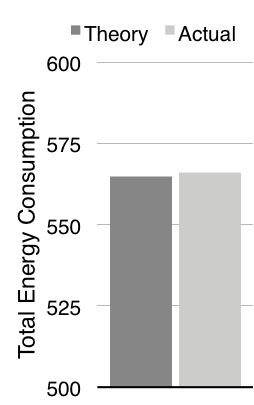
\includegraphics[scale=0.68]{testbed-p-hn250.png}}\hspace{0.3in}
		\subfigure[$U_{tot}=25, n = 250$ BaB-A]{\label{fig:tbabu25n250}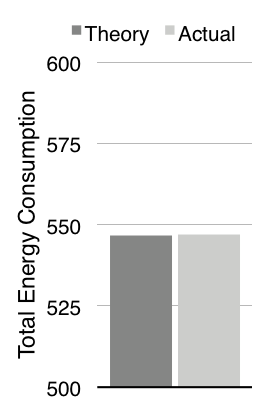
\includegraphics[scale=0.68]{testbed-p-bn250.png}}\hspace{0.3in}
		\subfigure[$U_{tot}=25, n = 450$ HyWGA]{\label{fig:thwgu25n450}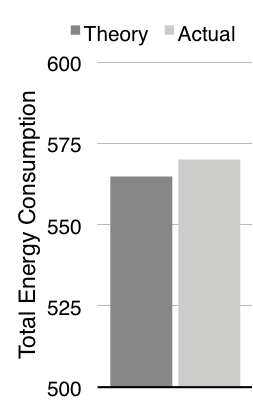
\includegraphics[scale=0.68]{testbed-p-hn450.png}}\hspace{0.3in}
		\subfigure[$U_{tot}=25, n = 450$ BaB-A]{\label{fig:tbabu25n450}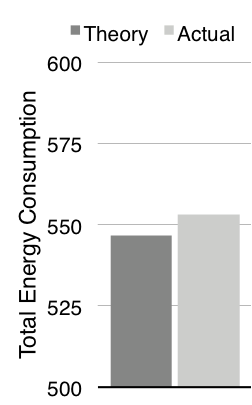
\includegraphics[scale=0.68]{testbed-p-bn450.png}}
	\end{center}
	\vspace{-0.12in}
		\caption{Theoretical vs. Actual Power Consumption on Testbed Cluster}
	\label{fig:testbed-res}
%\vspace{-0.15in}
\end{figure*}


With the power model confirmed we compare the performance of BaB-A and HyWGA by generating a set of task sets, applying the algorithms and comparing the schedules.
Maximum temperature is randomly selected as a value between $40-50^{\circ}$C. 9 different task sets are generated with the maximum utilization $U_{tot}$ set to $25$, $35$, and $45$ and the number of tasks $n$ set to $250$, $350$, and $450$ respectively.
Maximum task size is used to increment $U_{min}$ in BaB-A (Alg.~\ref{alg:bab}).
Each task set is run 10 times each to find a standard error, standard deviation is used to determine the standard error. Results are shown in Figs.~\ref{fig:theory-res}. We can see a clear improvement of BaB-A over the HyWGA, with a difference up to $3.25$\%. For the task sets with a $U_{tot} = 45$ the improvement is between $0.36$ and $0.74$\% (Figs.~\ref{fig:shu25}-\ref{fig:shu45}), to further investigate why this was we look at the testbed cluster.
Due to our testbed cluster being fairly homogeneous the selection of cores becomes less important to improve the schedule, a good schedule can be found by minimizing the number of cores used. The maximum improvement can therefore never exceed the power consumption of adding another processor, regardless of the size of $U_{tot}$. This makes not only a measurement in percentage improvement misleading, as $U_{tot}$ goes up, but can also for certain task sets give a close to optimal solution using HyWGA.
By using a value of power consumption instead of percentage for improvement difference we get improvements ranging from $3.64$ to $21.99$W. This result is still not good enough for the minimum improvement. To see if the problem is with the cluster being too homogeneous we tweak the testbed, making it more heterogenenous, this should then give a more general performance improvement to our algorithm. The results shown in Figs.~\ref{fig:stu25}-\ref{fig:stu45} show that this is the case with performance improvements ranging from $23.92$ to $45.43$W, a much more general improvement.
This shows that the power of our algorithm lies in it being dynamic enough to handle clusters where there are significant differences in processors.

\begin{figure*}[!t]
%\vspace{-0.12in}
	\begin{center}
		\subfigure[$U_{tot}=25$]{\label{fig:stu25}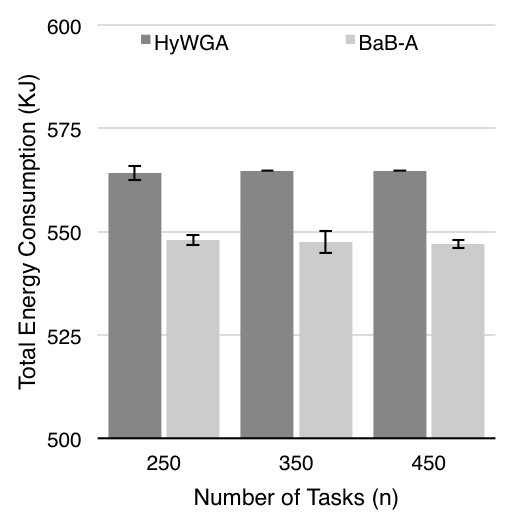
\includegraphics[scale=0.60]{simt-p-u25.png}}
		\subfigure[$U_{tot}=35$]{\label{fig:stu35}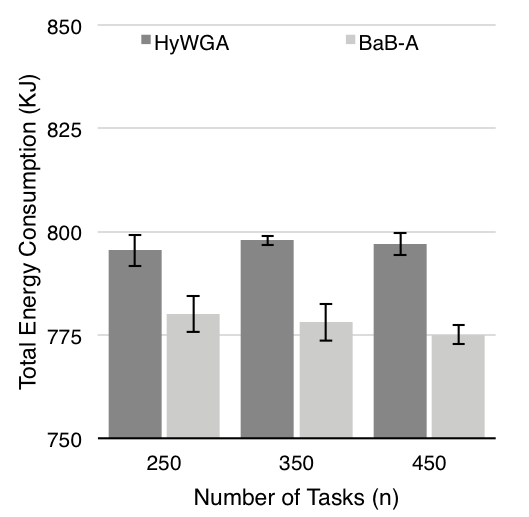
\includegraphics[scale=0.60]{simt-p-u35.png}}
		\subfigure[$U_{tot}=45$]{\label{fig:stu45}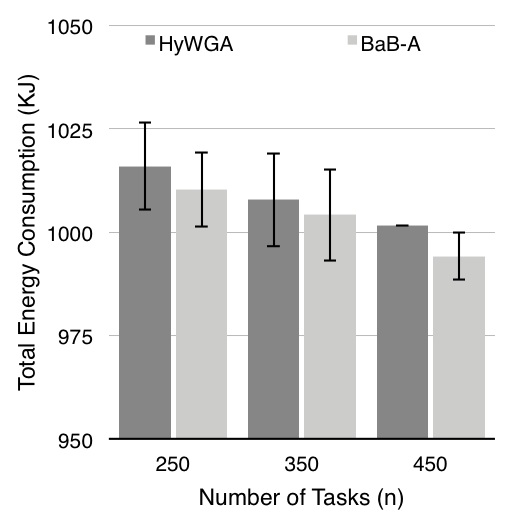
\includegraphics[scale=0.60]{simt-p-u45.png}}
	\end{center}
	\vspace{-0.12in}
		\caption{Theoretical Total Power Consumption for Testbed Cluster}
	\label{fig:theory-res}
%\vspace{-0.15in}
\end{figure*}

\begin{figure*}[!t]
%\vspace{-0.12in}
	\begin{center}
		\subfigure[$U_{tot}=25$]{\label{fig:shu25}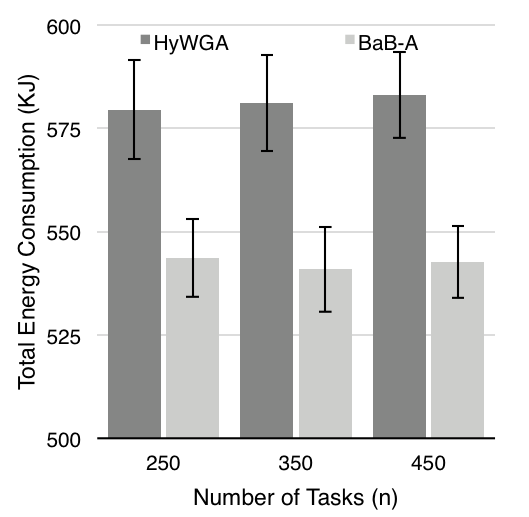
\includegraphics[scale=0.60]{simh-p-u25.png}}
		\subfigure[$U_{tot}=35$]{\label{fig:shu35}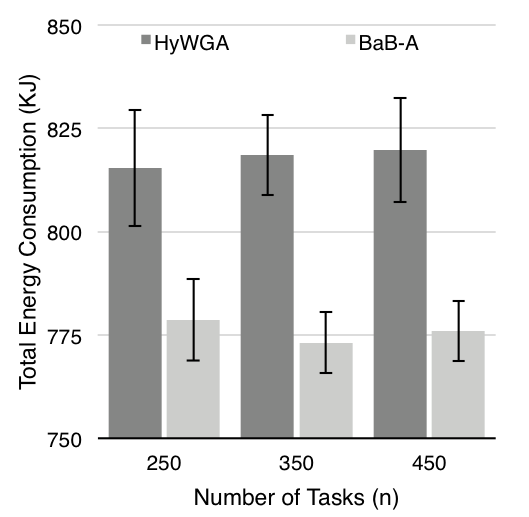
\includegraphics[scale=0.60]{simh-p-u35.png}}
		\subfigure[$U_{tot}=45$]{\label{fig:shu45}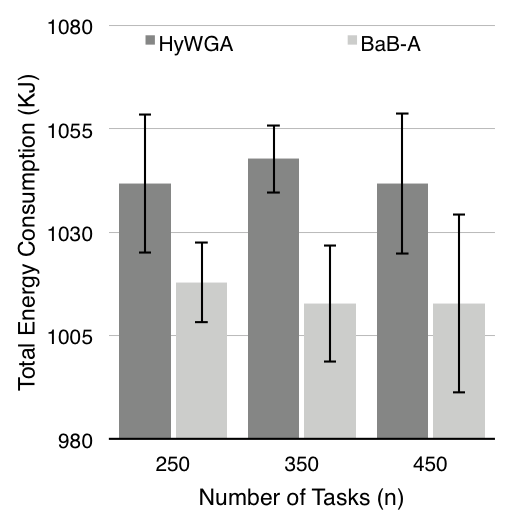
\includegraphics[scale=0.60]{simh-p-u45.png}}
	\end{center}
	\vspace{-0.12in}
		\caption{Theoretical Total Power Consumption for Heterogeneous Cluster}
	\label{fig:hetero-res}
%\vspace{-0.15in}
\end{figure*}

\bibliography{ipccc14}
\bibliographystyle{ieeetr}

%
%\begin{thebibliography}{00}
%\end{thebibliography}

\end{document}
